\documentclass[12pt,twoside]{article}

\newcommand{\reporttitle}{Maths for Machine Learning}
\newcommand{\reportauthor}{Alexander Gaskell}
\newcommand{\reporttype}{Coursework 3}
\newcommand{\cid}{01813313}

% include files that load packages and define macros
%%%%%%%%%%%%%%%%%%%%%%%%%%%%%%%%%%%%%%%%%
% University Assignment Title Page 
% LaTeX Template
% Version 1.0 (27/12/12)
%
% This template has been downloaded from:
% http://www.LaTeXTemplates.com
%
% Original author:
% WikiBooks (http://en.wikibooks.org/wiki/LaTeX/Title_Creation)
%
% License:
% CC BY-NC-SA 3.0 (http://creativecommons.org/licenses/by-nc-sa/3.0/)
% 
% Instructions for using this template:
% This title page is capable of being compiled as is. This is not useful for 
% including it in another document. To do this, you have two options: 
%
% 1) Copy/paste everything between \begin{document} and \end{document} 
% starting at \begin{titlepage} and paste this into another LaTeX file where you 
% want your title page.
% OR
% 2) Remove everything outside the \begin{titlepage} and \end{titlepage} and 
% move this file to the same directory as the LaTeX file you wish to add it to. 
% Then add \input{./title_page_1.tex} to your LaTeX file where you want your
% title page.
%
%----------------------------------------------------------------------------------------
%	PACKAGES AND OTHER DOCUMENT CONFIGURATIONS
%----------------------------------------------------------------------------------------
\usepackage{ifxetex}
\usepackage{textpos}
\usepackage{natbib}
\usepackage{kpfonts}
\usepackage[a4paper,hmargin=2.8cm,vmargin=2.0cm,includeheadfoot]{geometry}
\usepackage{ifxetex}
\usepackage{stackengine}
\usepackage{tabularx,longtable,multirow,subfigure,caption}%hangcaption
\usepackage{fncylab} %formatting of labels
\usepackage{fancyhdr}
\usepackage{color}
\usepackage[tight,ugly]{units}
\usepackage{url}
\usepackage{float}
\usepackage[english]{babel}
\usepackage{amsmath}
\usepackage{graphicx}
\usepackage[colorinlistoftodos]{todonotes}
\usepackage{dsfont}
\usepackage{epstopdf} % automatically replace .eps with .pdf in graphics
\usepackage{natbib}
\usepackage{backref}
\usepackage{array}
\usepackage{latexsym}
\usepackage{etoolbox}

\usepackage{enumerate} % for numbering with [a)] format 



\ifxetex
\usepackage{fontspec}
\setmainfont[Scale=.8]{OpenDyslexic-Regular}
\else
\usepackage[pdftex,pagebackref,hypertexnames=false,colorlinks]{hyperref} % provide links in pdf
\hypersetup{pdftitle={},
  pdfsubject={}, 
  pdfauthor={\reportauthor},
  pdfkeywords={}, 
  pdfstartview=FitH,
  pdfpagemode={UseOutlines},% None, FullScreen, UseOutlines
  bookmarksnumbered=true, bookmarksopen=true, colorlinks,
    citecolor=black,%
    filecolor=black,%
    linkcolor=black,%
    urlcolor=black}
\usepackage[all]{hypcap}
\fi

\usepackage{tcolorbox}

% various theorems
\usepackage{ntheorem}
\theoremstyle{break}
\newtheorem{lemma}{Lemma}
\newtheorem{theorem}{Theorem}
\newtheorem{remark}{Remark}
\newtheorem{definition}{Definition}
\newtheorem{proof}{Proof}

% example-environment
\newenvironment{example}[1][]
{ 
\vspace{4mm}
\noindent\makebox[\linewidth]{\rule{\hsize}{1.5pt}}
\textbf{Example #1}\\
}
{ 
\noindent\newline\makebox[\linewidth]{\rule{\hsize}{1.0pt}}
}



%\renewcommand{\rmdefault}{pplx} % Palatino
% \renewcommand{\rmdefault}{put} % Utopia

\ifxetex
\else
\renewcommand*{\rmdefault}{bch} % Charter
\renewcommand*{\ttdefault}{cmtt} % Computer Modern Typewriter
%\renewcommand*{\rmdefault}{phv} % Helvetica
%\renewcommand*{\rmdefault}{iwona} % Avant Garde
\fi

\setlength{\parindent}{0em}  % indentation of paragraph

\setlength{\headheight}{14.5pt}
\pagestyle{fancy}
\fancyfoot[ER,OL]{\thepage}%Page no. in the left on
                                %odd pages and on right on even pages
\fancyfoot[OC,EC]{\sffamily }
\renewcommand{\headrulewidth}{0.1pt}
\renewcommand{\footrulewidth}{0.1pt}
\captionsetup{margin=10pt,font=small,labelfont=bf}


%--- chapter heading

\def\@makechapterhead#1{%
  \vspace*{10\p@}%
  {\parindent \z@ \raggedright %\sffamily
        %{\Large \MakeUppercase{\@chapapp} \space \thechapter}
        %\\
        %\hrulefill
        %\par\nobreak
        %\vskip 10\p@
    \interlinepenalty\@M
    \Huge \bfseries 
    \thechapter \space\space #1\par\nobreak
    \vskip 30\p@
  }}

%---chapter heading for \chapter*  
\def\@makeschapterhead#1{%
  \vspace*{10\p@}%
  {\parindent \z@ \raggedright
    \sffamily
    \interlinepenalty\@M
    \Huge \bfseries  
    #1\par\nobreak
    \vskip 30\p@
  }}
  



% %%%%%%%%%%%%% boxit
\def\Beginboxit
   {\par
    \vbox\bgroup
	   \hrule
	   \hbox\bgroup
		  \vrule \kern1.2pt %
		  \vbox\bgroup\kern1.2pt
   }

\def\Endboxit{%
			      \kern1.2pt
		       \egroup
		  \kern1.2pt\vrule
		\egroup
	   \hrule
	 \egroup
   }	

\newenvironment{boxit}{\Beginboxit}{\Endboxit}
\newenvironment{boxit*}{\Beginboxit\hbox to\hsize{}}{\Endboxit}



\allowdisplaybreaks

\makeatletter
\newcounter{elimination@steps}
\newcolumntype{R}[1]{>{\raggedleft\arraybackslash$}p{#1}<{$}}
\def\elimination@num@rights{}
\def\elimination@num@variables{}
\def\elimination@col@width{}
\newenvironment{elimination}[4][0]
{
    \setcounter{elimination@steps}{0}
    \def\elimination@num@rights{#1}
    \def\elimination@num@variables{#2}
    \def\elimination@col@width{#3}
    \renewcommand{\arraystretch}{#4}
    \start@align\@ne\st@rredtrue\m@ne
}
{
    \endalign
    \ignorespacesafterend
}
\newcommand{\eliminationstep}[2]
{
    \ifnum\value{elimination@steps}>0\leadsto\quad\fi
    \left[
        \ifnum\elimination@num@rights>0
            \begin{array}
            {@{}*{\elimination@num@variables}{R{\elimination@col@width}}
            |@{}*{\elimination@num@rights}{R{\elimination@col@width}}}
        \else
            \begin{array}
            {@{}*{\elimination@num@variables}{R{\elimination@col@width}}}
        \fi
            #1
        \end{array}
    \right]
    & 
    \begin{array}{l}
        #2
    \end{array}
    &%                                    moved second & here
    \addtocounter{elimination@steps}{1}
}
\makeatother

%% Fast macro for column vectors
\makeatletter  
\def\colvec#1{\expandafter\colvec@i#1,,,,,,,,,\@nil}
\def\colvec@i#1,#2,#3,#4,#5,#6,#7,#8,#9\@nil{% 
  \ifx$#2$ \begin{bmatrix}#1\end{bmatrix} \else
    \ifx$#3$ \begin{bmatrix}#1\\#2\end{bmatrix} \else
      \ifx$#4$ \begin{bmatrix}#1\\#2\\#3\end{bmatrix}\else
        \ifx$#5$ \begin{bmatrix}#1\\#2\\#3\\#4\end{bmatrix}\else
          \ifx$#6$ \begin{bmatrix}#1\\#2\\#3\\#4\\#5\end{bmatrix}\else
            \ifx$#7$ \begin{bmatrix}#1\\#2\\#3\\#4\\#5\\#6\end{bmatrix}\else
              \ifx$#8$ \begin{bmatrix}#1\\#2\\#3\\#4\\#5\\#6\\#7\end{bmatrix}\else
                 \PackageError{Column Vector}{The vector you tried to write is too big, use bmatrix instead}{Try using the bmatrix environment}
              \fi
            \fi
          \fi
        \fi
      \fi
    \fi
  \fi 
}  
\makeatother

\robustify{\colvec}

%%% Local Variables: 
%%% mode: latex
%%% TeX-master: "notes"
%%% End: 
 % various packages needed for maths etc.
% quick way of adding a figure
\newcommand{\fig}[3]{
 \begin{center}
 \scalebox{#3}{\includegraphics[#2]{#1}}
 \end{center}
}

%\newcommand*{\point}[1]{\vec{\mkern0mu#1}}
\newcommand{\ci}[0]{\perp\!\!\!\!\!\perp} % conditional independence
\newcommand{\point}[1]{{#1}} % points 
\renewcommand{\vec}[1]{{\boldsymbol{{#1}}}} % vector
\newcommand{\mat}[1]{{\boldsymbol{{#1}}}} % matrix
\newcommand{\R}[0]{\mathds{R}} % real numbers
\newcommand{\Z}[0]{\mathds{Z}} % integers
\newcommand{\N}[0]{\mathds{N}} % natural numbers
\newcommand{\nat}[0]{\mathds{N}} % natural numbers
\newcommand{\Q}[0]{\mathds{Q}} % rational numbers
\ifxetex
\newcommand{\C}[0]{\mathds{C}} % complex numbers
\else
\newcommand{\C}[0]{\mathds{C}} % complex numbers
\fi
\newcommand{\tr}[0]{\text{tr}} % trace
\renewcommand{\d}[0]{\mathrm{d}} % total derivative
\newcommand{\inv}{^{-1}} % inverse
\newcommand{\id}{\mathrm{id}} % identity mapping
\renewcommand{\dim}{\mathrm{dim}} % dimension
\newcommand{\rank}[0]{\mathrm{rk}} % rank
\newcommand{\determ}[1]{\mathrm{det}(#1)} % determinant
\newcommand{\scp}[2]{\langle #1 , #2 \rangle}
\newcommand{\kernel}[0]{\mathrm{ker}} % kernel/nullspace
\newcommand{\img}[0]{\mathrm{Im}} % image
\newcommand{\idx}[1]{{(#1)}}
\DeclareMathOperator*{\diag}{diag}
\newcommand{\E}{\mathds{E}} % expectation
\newcommand{\var}{\mathds{V}} % variance
\newcommand{\gauss}[2]{\mathcal{N}\big(#1,\,#2\big)} % gaussian distribution N(.,.)
\newcommand{\gaussx}[3]{\mathcal{N}\big(#1\,|\,#2,\,#3\big)} % gaussian distribution N(.|.,.)
\newcommand{\gaussBig}[2]{\mathcal{N}\left(#1,\,#2\right)} % see above, but with brackets that adjust to the height of the arguments
\newcommand{\gaussxBig}[3]{\mathcal{N}\left(#1\,|\,#2,\,#3\right)} % see above, but with brackets that adjust to the height of the arguments
\DeclareMathOperator{\cov}{Cov} % covariance (matrix) 
\ifxetex
\renewcommand{\T}[0]{^\top} % transpose
\else
\newcommand{\T}[0]{^\top}
\fi
% matrix determinant
\newcommand{\matdet}[1]{
\left|
\begin{matrix}
#1
\end{matrix}
\right|
}



%%% various color definitions
\definecolor{darkgreen}{rgb}{0,0.6,0}

\newcommand{\blue}[1]{{\color{blue}#1}}
\newcommand{\red}[1]{{\color{red}#1}}
\newcommand{\green}[1]{{\color{darkgreen}#1}}
\newcommand{\orange}[1]{{\color{orange}#1}}
\newcommand{\magenta}[1]{{\color{magenta}#1}}
\newcommand{\cyan}[1]{{\color{cyan}#1}}


% redefine emph
\renewcommand{\emph}[1]{\blue{\bf{#1}}}

% place a colored box around a character
\gdef\colchar#1#2{%
  \tikz[baseline]{%
  \node[anchor=base,inner sep=2pt,outer sep=0pt,fill = #2!20] {#1};
    }%
}%
 % short-hand notation and macros

\renewcommand{\thesubsection}{\thesection.\alph{subsection}}

%%%%%%%%%%%%%%%%%%%%%%%%%%%%

\begin{document}
% front page
% Last modification: 2016-09-29 (Marc Deisenroth)
\begin{titlepage}

\newcommand{\HRule}{\rule{\linewidth}{0.5mm}} % Defines a new command for the horizontal lines, change thickness here


%----------------------------------------------------------------------------------------
%	LOGO SECTION
%----------------------------------------------------------------------------------------


\includegraphics[width = 4cm]{./figures/imperial}\\[0.5cm] 

\begin{center} % Center remainder of the page

%----------------------------------------------------------------------------------------
%	HEADING SECTIONS
%----------------------------------------------------------------------------------------
\textsc{\LARGE \reporttype}\\[1.5cm] 
\textsc{\Large Imperial College London}\\[0.5cm] 
\textsc{\large Department of Computing}\\[0.5cm] 
%----------------------------------------------------------------------------------------
%	TITLE SECTION
%----------------------------------------------------------------------------------------

\HRule \\[0.4cm]
{ \huge \bfseries \reporttitle}\\ % Title of your document
\HRule \\[1.5cm]
\end{center}
%----------------------------------------------------------------------------------------
%	AUTHOR SECTION
%----------------------------------------------------------------------------------------

%\begin{minipage}{0.4\hsize}
\begin{flushleft} \large
\textit{Author:}\\
\reportauthor~(CID: \cid) \\% Your name 
\textit{Email:} \\
\reportemail
\end{flushleft}
\vspace{2cm}
\makeatletter
Date: \@date 

\vfill % Fill the rest of the page with whitespace



\makeatother


\end{titlepage}




%%%%%%%%%%%%%%%%%%%%%%%%%%%% Main document
\section{}

\subsection{}
\textbf{[5 marks] By first finding the maximum likelihood solution for the parameters $\sigma^2$ and $w$ in terms of $\Phi$, plot the predicted mean at test points in the interval $[-0.3, 1.3]$ in the case of polynomial basis functions of order $0, 1, 2, 3$ and order $11$. Plot all the curves on the same axes, showing also the data.}
\bigbreak
The maximum likelihood estimator is found by the following (As per the Piazza question I will not derive this result):
\begin{align}
    \mathbf{\theta_{ML} = (\Phi^\top \Phi)^{-1}\Phi^\top y}
\end{align}
Where $\mathbf{\Phi}$ is the design matrix, and is defined by:
\begin{align}=
    \mathbf{\Phi} = \colvec{\phi^\top(\mathbf{x}_1),\vdots,\phi^\top (\mathbf{x}_N)} = \begin{bmatrix} 
    \phi_0(\mathbf{x}_1) & ... & \phi_{K-1}(\mathbf{x}_1) \\ \vdots & \ddots & \vdots \\ \phi_0(\mathbf{x}_N) & ... & \phi_{K-1}(\mathbf{x}_N)
    \end{bmatrix} \in \mathbb{R}^{NxK}
\end{align}

The max likelihood value for $\sigma^2$ can be derived as follows:
\begin{align}
    \operatorname{log} p(\mathcal{Y} | \mathcal{X}, \boldsymbol{\theta}, \sigma^2) 
    & = \sum^{N}_{n=1} \operatorname{log} \mathcal{N} (y_n | \mathbf{w}^\top \boldsymbol{\phi}(x_i), \sigma^2) \\
    & = \sum^{N}_{n=1} 
    \begin{pmatrix} 
    -\frac{1}{2} \operatorname{log}(2\pi) - \frac{1}{2} \operatorname{log} \sigma^2 -\frac{1}{2\sigma^2}(y_n - \mathbf{w}^\top \boldsymbol{\phi}(x_i))^2
    \end{pmatrix} \\
    & = -\frac{N}{2} \operatorname{log} \sigma^2 - \frac{1}{2\sigma^2} \sum^{N}_{n=1} (y_n - \mathbf{w}^\top \boldsymbol{\phi}(x_i))^2 + \operatorname{constant} \\
    & = -\frac{N}{2} \operatorname{log} \sigma^2 - \frac{s}{2\sigma^2} + \operatorname{constant}
\end{align}

Differentiate with respect to $\sigma^2$ and set equal to zero to find the maximum:

\begin{align}
    & \frac{\partial \operatorname{log} p(\mathcal{Y} | \mathcal{X}, \boldsymbol{\theta}, \sigma^2)}{\partial \sigma^2} = -\frac{N}{2\sigma^2} + \frac{s}{2\sigma^4} = 0 \\
    & \iff \frac{N}{2\sigma^2} = \frac{s}{2\sigma^4}
\end{align}

This gives our maximum likelihood estimate for $\sigma^2$:

\begin{align}
    \sigma^2_{ML} = \frac{s}{N} = \frac{1}{N}\sum^{N}_{n=1} (y_n - \mathbf{w}^\top \boldsymbol{\phi}(x_i))^2
\end{align}

\begin{figure}[h]
\centering % this centers the figure
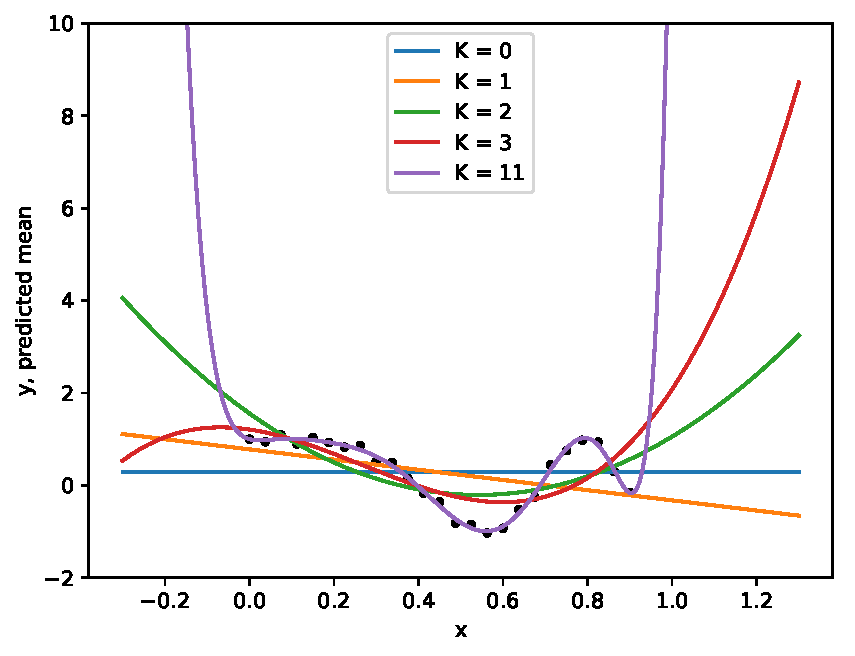
\includegraphics[width = 0.9\hsize] {./figures/polynomial.pdf}
\caption{Plots of generated data points and the predicted means of polynomial basis functions of orders 0,1,2,3,11 (K = order of basis function)}% caption of the figure
\label{fig:poly}
\end{figure}





\subsection{}
\textbf{[5 marks] Repeat the previous part but this time with trigonometric basis functions of orders 1 and 11. Use test points in $[-1, 1.2]$ to see the periodicity. Note that your basis functions should be of size $2J + 1$ for order $J$ (i.e., don’t forget the bias term)}
\\

See figure \ref{fig:trig} for illustration.

\begin{figure}[h]
\centering % this centers the figure
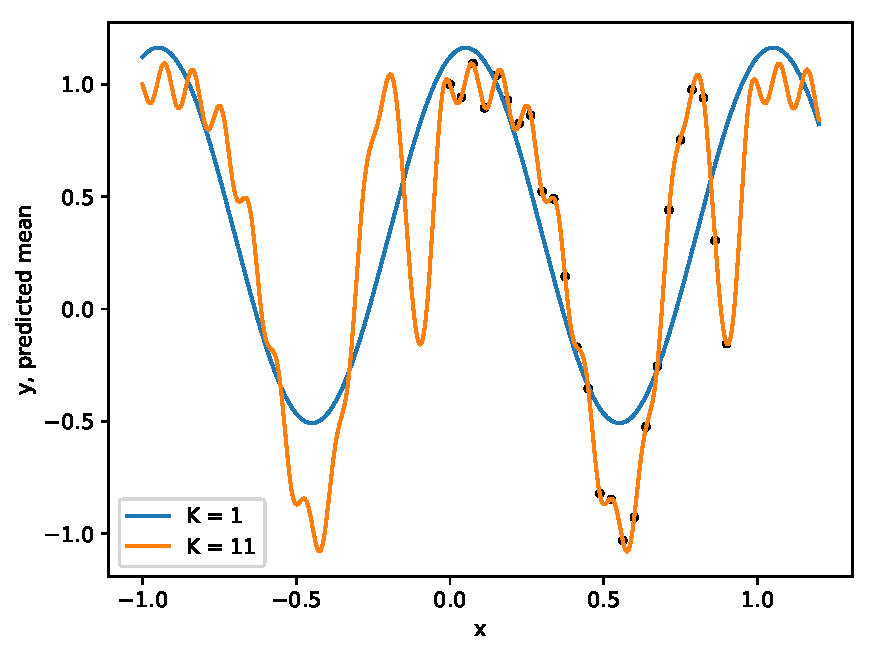
\includegraphics[width = 0.9\hsize] {./figures/trigonometric.pdf}
\caption{Plots of generated data points and the predicted means of trigonometric basis functions of orders 1,11 (K = order of basis function)}% caption of the figure
\label{fig:trig}
\end{figure}

\newpage


\subsection{}
\textbf{[6 marks] In this part, you will investigate over-fitting with leave-one- out cross validation. You should use trigonometric basis functions of order 0 to 10 inclusive. For each choice, use leave-one-out cross-validation to estimate the average squared test error. Plot this average error on a graph against order of basis together. On the same graph plot also the maximum likelihood value for $\sigma$.}
\\ \\
See figure \ref{fig:error} for illustration.

\begin{figure}[h]
\centering % this centers the figure
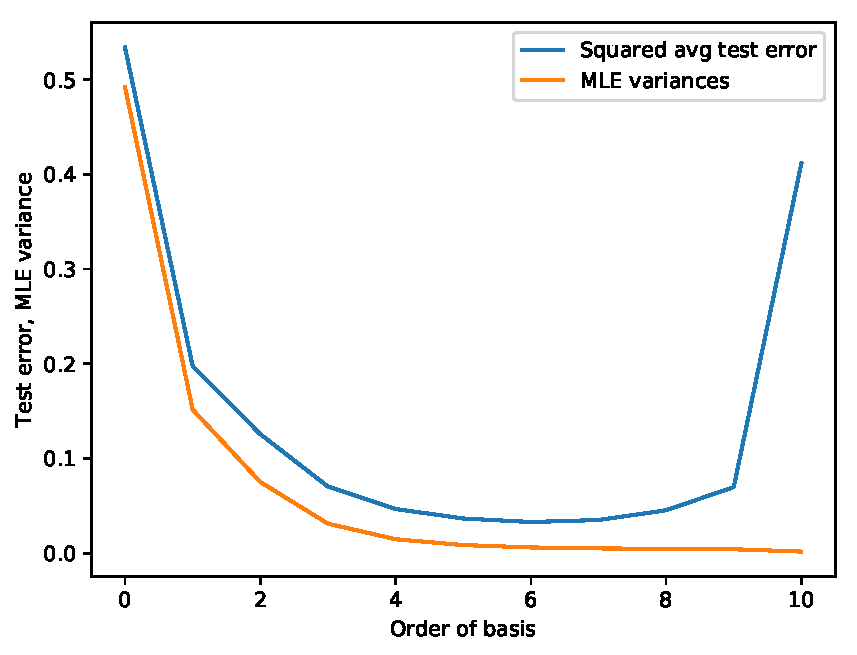
\includegraphics[width = 0.9\hsize] {./figures/sq_error_variance.pdf}
\caption{Plots of generated data points and the predicted means of trigonometric basis functions of orders 0,1,2,3,11}% caption of the figure
\label{fig:error}
\end{figure}

\newpage

\subsection{}
\textbf{[6 marks] Briefly describe the concept of over-fitting, using your graph in the previous part as an illustrative example. You should also refer to your plots from the first two parts of this question.}\\

Overfitting is when the model fits the training data too closely and consequently does not generalise unseen data well. Specifically, overfitting occurs when the empirical error observed on the training data underestimates the true error of the model. \\

This is well illustrated in figure \ref{fig:error}:
the x-axis is the order of basis ($K$) of the trigonometric basis functions, so can be thought of as the "complexity" of the model. The squared errors are obtained from leave-one-out cross validation, so represent the true/test error of the model, and the variances are the maximum likelihood variance estimations, so represent the training error of the model. The plots begin by moving in tandem with both training and test error falling. This is because the model initially underfits when the order of the basis functions is low. However, test and training error diverge once order of basis exceeds 6, hence overfitting starts becoming a problem for $K \geq 6$. \\

This occurs because increasing the complexity of the model means the model has more free parameters and can therefore approximate a larger number of functions well. Consequently, fitting a more complex model to the same training data set will mean the model will always fit the data better (than a less complex version of that model), hence the training error will always fall if when the complexity of the model rises. However, at a certain point, increasing the complexity of the model will give it sufficient free parameters to model noise in the training data, which is not generalizable given it is random. This is why we see the test error rising when order of basis is increased above 6. \\

Overfitting can also be seen in figures \ref{fig:poly} and \ref{fig:trig}: beginning from $K=0$, if we increase $K$ then the plot does a better job of of fitting the data points; however, once we set $K=11$, the model does a very good job of hitting every data point but has poor generalisation properties. This can be seen for $K=11$, figure \ref{fig:poly}, with the tails of the plot shooting nearly vertically upwards. Additionally, for $K=11$, figure \ref{fig:trig}, the model appears to follow noise in the data, and so it is unlikely that this model would generalise better to new data than a smoother, lower-order trigonometric model. In both of these cases, the model performs well on the training data but would perform poorly on unseen data, so this illustrates clearly the concept of overfitting.

\newpage

\section{}

\subsection{}
\textbf{[6 marks] Write a python function lml(alpha, beta, Phi, Y) that returns the log-marginal likelihood, and a function grad\_lml(alpha, beta, Phi, Y) that returns the gradient of the log-marginal likelihood with respect to the vector $[\alpha, \beta]$.}


\subsection{}
\textbf{[6 marks] For the given dataset and the linear basis functions (i.e., polynomial of order 1), maximize the log-marginal likelihood with respect to $\alpha$ and $\beta$ using gradient descent. Show your steps on a contour plot. It is up to you, where you start, but be careful that the log-marginal likelihood varies over several orders of magnitude, so you may have to start fairly close. You may have to clip your contours to show anything interesting on the plot. Don’t use a log-scale for $\alpha$ and $\beta$ (though this would be sensible). Report your results for the maximum.} \\

Convergence results: $\alpha = 0.425, \beta = 0.450$

\begin{figure}[h]
\centering % this centers the figure
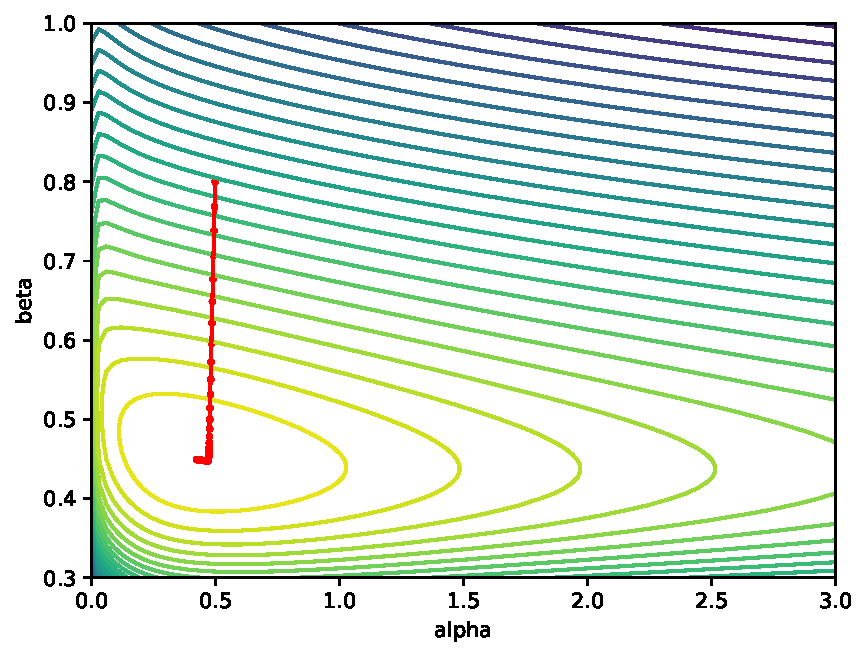
\includegraphics[width = 0.9\hsize] {./figures/log_marginal_likelihood.pdf}
\caption{Contour plot of log marginal likelihood with }% caption of the figure
\label{fig:log_marginal_likelihood}
\end{figure}



\subsection{}
\textbf{[3 marks] In the case of trigonometric basis functions, compute the maximum of the log-marginal likelihood for orders 0 to 12 inclusive using gradient descent (make sure you choose good starting values and a small step size with plenty of iterations). Plot these values on a graph against the order of the basis functions. Compare your answer to your cross-validation graph in question 1c) and describe briefly the merits of the two approaches.}\\

The results from figure \ref{fig:basis_vs_max_mar_likeli} are consistent with those of the cross-validation graph in figure \ref{fig:error} in that they both initially show underfitting (the max log marginal likelihood is rising until order of basis = 4), then they level off, and then they show overfitting when order of basis is above 6. This is unsurprising given that maximising the log marginal likelihood is an alternative method of model selection to cross validation. The marginal likelihood encapsulates the trade off between increasing model complexity with fit of the data, in that it "penalises" models which are too complex. This penalty is what makes the log marginal likelihood fall for order of basis above 6, analogously to the way that the test error rises when using cross validation because more complex functions often do not generalise as well as less complex functions.


\begin{figure}[h]
\centering % this centers the figure
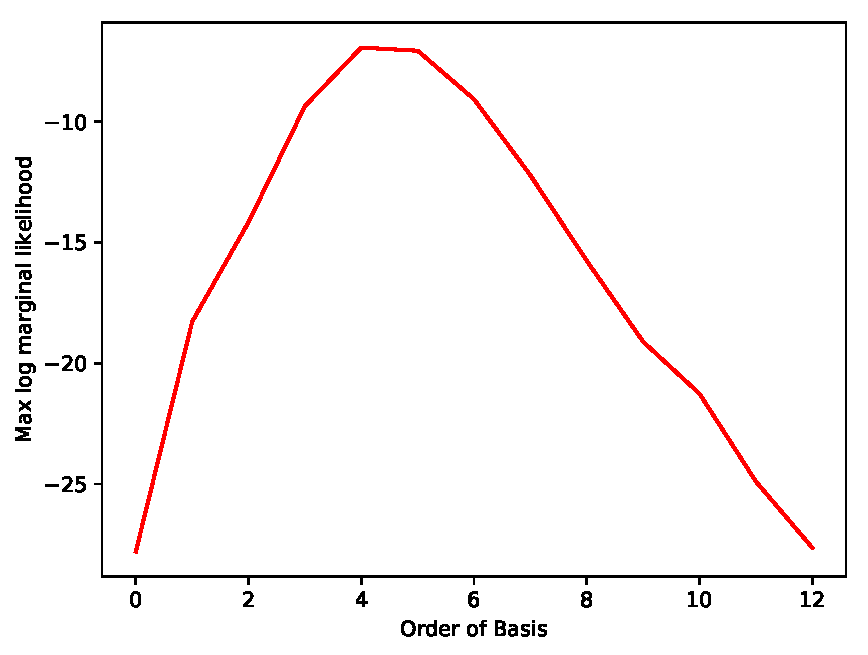
\includegraphics[width = 0.9\hsize] {./figures/basis_vs_max_mar_likeli.pdf}
\caption{Plot of max of log marginal likelihood vs order of basis (using trigonometric basis functions)}% caption of the figure
\label{fig:basis_vs_max_mar_likeli}
\end{figure}



\subsection{}
\textbf{[8 marks] For $\alpha = 1$ and $\beta = 0.1$ take 5 samples from the posterior distribution over the weights in the case of 10 Gaussian basis functions equally spaced between −0.5 and 1 (inclusive) with scale 0.1. Use these samples to plot the noise-free predicted function values at the test points (i.e., with y-values $\mathbf{\Phi^*w}$, where $\mathbf{\Phi^*}$ is the matrix of stacked basis functions evaluated at the test inputs $x^*$). Plot also the predictive mean and 2 standard deviation error bars as a shaded region. Don’t include the noise in your shaded region, but do add also dotted curves indicating two standard deviations including the noise (i.e., dotted for $y^*$ and shaded for $\mathbf{\Phi^*w}$). Use test points in the interval $[−1, 1.5]$ to show the behavior away from the data and away from the basis function centers. Plot the samples in a different color and use a low alpha (in the sense of opacity!) for the shaded region. Plot also the data.}

\begin{figure}[h]
\centering % this centers the figure
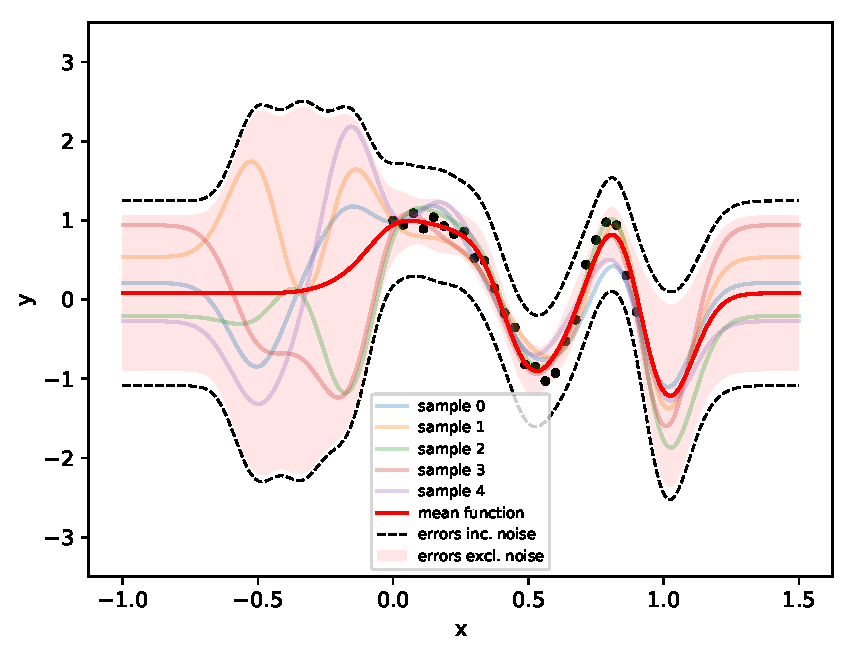
\includegraphics[width = 0.9\hsize] {./figures/exp_with_errs.pdf}
\caption{Plot of noise-free predicted function values $y^*$ using 5 samples taken from the posterior distribution over weights and the predictive mean. Additionally, error bars (2 standard deviations without noise) and error bars (2 standard deviations with noise) have been plotted above.}% caption of the figure
\label{fig:exp_with_errs}
\end{figure}





\end{document}
%%% Local Variables: 
%%% mode: latex
%%% TeX-master: t
%%% End: 
